\documentclass[11pt]{article}

\usepackage[a4paper,margin=1in]{geometry}
\usepackage[T1]{fontenc}
\usepackage[utf8]{inputenc}
\usepackage{lmodern}
\usepackage{microtype}
\usepackage{amsmath,amssymb,amsthm,mathtools}
\usepackage{booktabs,array}
\usepackage{graphicx}
\usepackage{float}
\usepackage[section]{placeins}
\usepackage{enumitem}
\usepackage[numbers,sort&compress]{natbib}
\usepackage{xcolor}
\usepackage{xurl}
\usepackage[colorlinks=true,linkcolor=blue!55!black,citecolor=blue!55!black,urlcolor=blue!55!black]{hyperref}
\usepackage[nameinlink,noabbrev]{cleveref}

\newtheorem{theorem}{Theorem}[section]
\newtheorem{proposition}[theorem]{Proposition}
\newtheorem{lemma}[theorem]{Lemma}
\newtheorem{corollary}[theorem]{Corollary}
\theoremstyle{definition}
\newtheorem{definition}[theorem]{Definition}
\theoremstyle{remark}
\newtheorem{remark}[theorem]{Remark}

\newcommand{\Id}{I}
\newcommand{\Ac}{A_{\mathrm c}}
\newcommand{\Af}{A_{\mathrm f}}
\newcommand{\GammaC}{\Gamma}
\newcommand{\norm}[1]{\left\lVert #1\right\rVert}
\newcommand{\C}{\mathbb C}

\title{A Certified Nested-Grid Continuation of a Physical Spectral Count\\
\large Dyadic Schur Self-Energy and a \(2048\)-to-\(4096\) Dimension Transfer\\
at a Quadratic Band-Merging Map}
\author{Liang Wang}
\date{July 2026}

\begin{document}
\maketitle

\begin{abstract}
A preceding finite-model certificate proved that one exact stored
\(2048\)-dimensional Perron/parity-extracted physical two-step matrix has
exactly one eigenvalue inside a prescribed complex circle.  That theorem did
not show that the count survives grid refinement.  We give the first rigorous
adjacent-dimension continuation for this stored model, at fixed Gaussian noise
width \(\sigma=10^{-2}\), from \(2048\) to \(4096\) midpoint cells.

The fine grid is decomposed by exact dyadic replication and alternating-detail
coordinates.  Four rank-\(96\) stored approximants, certified by componentwise
factor-graph residuals, bound the coarse consistency, two cross channels, and
detail block by \(1.98878\times10^{-4}\), \(1.13215\times10^{-2}\),
\(1.37227\times10^{-2}\), and \(1.30523\times10^{-4}\), respectively.
The detail spectrum is excluded from the counting disk, and its Schur
self-energy is at most \(4.13077\times10^{-4}\).  Thus the fine effective
coarse block differs from the stored coarse physical matrix by at most
\(6.11954\times10^{-4}\) on the full contour.

A sparse-Grushin atlas with \(170\) rigorous centers and an exact
\(314\)-leaf rational partition bounds the matrix Rouch\'e product by
\(0.899350<1\).  A bitwise replay identifies the coarse object with the
preceding one-count certificate.  Consequently, for the exact stored
binary64 matrices,
\[
 \boxed{N_{\Gamma}(A_{2048})=N_{\Gamma}(A_{4096})=1.}
\]
This is a finite stored-matrix theorem at one fixed noise scale.  It is not a
continuum, arbitrary-dimension, or zero-noise result.
\end{abstract}

\section{Introduction}

Finite-dimensional spectral discoveries become mathematically useful only
after two logically separate questions are answered.  First, does a specified
stored matrix really have the reported contour count?  Second, does that count
survive a change of discretization?  The first question was closed for the
\(2048\)-dimensional physical two-step matrix in
\citet{WangPacketPair2026}.  The second remained open.

The distinction is substantial for nonnormal transfer matrices.  A visually
stable eigenvalue and a small entrywise grid change do not imply a stable
spectral count; the relevant amplification is controlled by the resolvent
\citep{Kato1995,TrefethenEmbree2005}.  Moreover, matrices at different
dimensions do not live in the same coordinate space.  A subtraction becomes
meaningful only after a lifting, restriction, and detail space are specified.

This paper fixes the Gaussian width at
\[
 \sigma=10^{-2}
\]
and compares the exact stored midpoint matrices at dimensions
\[
 n=2048,\qquad 2n=4096.
\]
The refinement is dyadic, so the fine space admits an exact binary
coarse/detail splitting.  The main mechanism is
\[
 \begin{gathered}
 \text{fine matrix}\longrightarrow\text{detail Schur complement}
 \longrightarrow\text{small analytic self-energy}\\
 \longrightarrow\text{coarse resolvent Rouch\'e comparison}.
 \end{gathered}
\]

Three technical points make the argument rigorous.
\begin{enumerate}[leftmargin=2em]
 \item The coordinate transform uses only copying, sign changes, and division
       by two.  No interpolation constant or irrational normalization enters
       the exact algebra.
 \item The four cross-grid blocks are not bounded by their Frobenius norms.
       Stored rank-\(96\) singular centers are combined with componentwise
       residual enclosures.  The centers are proof generators; the final
       inequalities include their full residuals.
 \item The coarse physical resolvent is certified directly.  A sparse
       two-step Grushin realization supplies approximate inverses, while exact
       stored-factor residuals convert them into rigorous bounds.
\end{enumerate}

The resulting theorem is a genuine discretization-stability step, but a
limited one.  It compares two finite stored matrices at one noise width.  It
does not establish a uniform \(n\to\infty\) estimate, despite the general
collectively compact framework for smooth integral kernels
\citep{Atkinson1997}.  It also does not move the noise parameter.

\section{Stored physical matrices and evidence levels}
\label{sec:model}

Let \(P_m\) denote the stored row-normalized folded Gaussian midpoint matrix
on \(m\) positive cells.  The deterministic map parameter, Gaussian cutoff,
row normalization, sparse indices, and all nonzero weights are archived in
the machine-readable snapshot.  Let
\[
 X_m,\ Y_m\in\mathbb R^{m\times2},\qquad
 \Lambda_m\in\mathbb R^{2\times2}
\]
be the stored right modes, left modes, and peripheral eigenvalue diagonal.
The Perron/parity-extracted one-step and physical two-step matrices are
\begin{equation}
 U_m=P_m-X_m\Lambda_mY_m^{T},
 \qquad A_m=U_m^2.
 \label{eq:physical}
\end{equation}
Every binary64 number in these factors is treated as an exact real number.
The theorem concerns
\[
 \Ac=A_{2048},\qquad \Af=A_{4096}.
\]

The counting contour is the positively oriented circle
\begin{equation}
 \GammaC:\quad z=z_0+r e^{i\theta},\qquad 0\le\theta\le2\pi,
 \label{eq:contour}
\end{equation}
with stored parameters
\begin{equation}
 z_0=-0.3233504401504541-0.5508412474453575i,
 \qquad r=0.2624987592858511.
 \label{eq:contour-values}
\end{equation}
The distance from the origin to the closed counting disk is bounded below by
\begin{equation}
 d_0=|z_0|-r\ge0.376235604149098.
 \label{eq:origin-distance}
\end{equation}

We distinguish three evidence levels.
\begin{description}[leftmargin=2.7cm,style=nextline]
 \item[Exact algebra]
 Coordinate identities and determinant factorizations over the exact stored
 real numbers.
 \item[Rigorous certificate]
 Outward bounds for the exact stored binary64 target under the stated
 round-to-nearest model, with Arb used for final scalar and circular-arc
 comparisons \citep{Johansson2017,Rump2010}.
 \item[Floating diagnostic]
 Sparse eigensolves and singular vectors used to choose proof objects and to
 display locations.  They do not establish the theorem.
\end{description}

\section{Exact dyadic coarse/detail coordinates}
\label{sec:coordinates}

For \(x,y\in\mathbb C^n\), define \(J,K:\mathbb C^n\to\mathbb C^{2n}\) by
\begin{align}
 (Jx)_{2j}&=(Jx)_{2j+1}=x_j,\label{eq:J}\\
 (Ky)_{2j}&=y_j,\qquad (Ky)_{2j+1}=-y_j.\label{eq:K}
\end{align}
Define
\begin{equation}
 R=\tfrac12J^T,\qquad S=\tfrac12K^T.
 \label{eq:RS}
\end{equation}
These are unnormalized Haar coarse/detail coordinates.  Their advantage is
exact representability in binary arithmetic.

\begin{lemma}[Exact dyadic inverse]
\label{lem:dyadic-inverse}
The maps satisfy
\[
 RJ=SK=\Id_n,\qquad RK=SJ=0,
\]
and therefore
\begin{equation}
 T=[J\ K],\qquad T^{-1}=\begin{pmatrix}R\\S\end{pmatrix}.
 \label{eq:T}
\end{equation}
\end{lemma}

\begin{proof}
Every identity follows independently on each fine-grid pair.  The sum of the
two replicated entries is \(2x_j\), while the difference of the alternating
entries is \(2y_j\).  The cross sum and cross difference vanish.
\end{proof}

In these coordinates write
\begin{equation}
 T^{-1}\Af T=
 \begin{pmatrix}
  A_{\rm cc}&B_{\rm cd}\\
  C_{\rm dc}&D_{\rm dd}
 \end{pmatrix},
 \label{eq:block-matrix}
\end{equation}
where
\begin{equation}
 A_{\rm cc}=R\Af J,\quad
 B_{\rm cd}=R\Af K,\quad
 C_{\rm dc}=S\Af J,\quad
 D_{\rm dd}=S\Af K.
 \label{eq:blocks}
\end{equation}
The coarse consistency defect is
\begin{equation}
 E_{\rm cc}=A_{\rm cc}-\Ac.
 \label{eq:Ecc}
\end{equation}

\begin{proposition}[Exact Schur determinant identity]
\label{prop:schur}
If \(z\Id-D_{\rm dd}\) is invertible, then
\begin{align}
 \det(z\Id_{2n}-\Af)
 &=\det(z\Id_n-D_{\rm dd})\det \mathcal F_{\rm f}(z),
 \label{eq:schur-det}\\
 \mathcal F_{\rm f}(z)
 &=z\Id_n-\Ac-\Delta(z),\label{eq:effective}\\
 \Delta(z)
 &=E_{\rm cc}+B_{\rm cd}(z\Id_n-D_{\rm dd})^{-1}C_{\rm dc}.
 \label{eq:self-energy}
\end{align}
\end{proposition}

\begin{proof}
Similarity by \(T\) preserves the characteristic determinant.  Taking the
Schur complement of the lower-right block in
\(z\Id-T^{-1}\Af T\) gives \eqref{eq:schur-det}.  Substituting
\(A_{\rm cc}=\Ac+E_{\rm cc}\) gives
\eqref{eq:effective}--\eqref{eq:self-energy}.
\end{proof}

\section{Certified low-rank bounds for the four blocks}
\label{sec:block-certificate}

Direct Frobenius estimates are insufficient.  The floating Frobenius
candidates for the two cross blocks are approximately \(4.23\times10^{-2}\)
and \(2.45\times10^{-2}\), whereas their spectral norms are about
\(1.13\times10^{-2}\) and \(1.37\times10^{-2}\).  This difference decides
whether the final Rouch\'e gate closes.

For each exact stored block \(E\), a floating sparse singular calculation
produces stored matrices
\[
 L\in\mathbb R^{n\times k},\qquad
 \Sigma=\operatorname{diag}(s_1,\ldots,s_k),\qquad
 V^T\in\mathbb R^{k\times n},
\]
with \(k=96\).  These arrays are not trusted as singular vectors.  They define
only an exact stored low-rank comparison matrix \(L\Sigma V^T\).

\begin{lemma}[Low-rank residual bound]
\label{lem:low-rank}
Suppose componentwise arithmetic proves
\[
 \norm{L^TL-\Id}_F\le\delta_L,\qquad
 \norm{VV^T-\Id}_F\le\delta_V,\qquad
 \norm{E-L\Sigma V^T}_F\le\rho.
\]
Then
\begin{equation}
 \norm{E}_2
 \le
 \sqrt{1+\delta_L}\,\max_j|s_j|\,
 \sqrt{1+\delta_V}+\rho.
 \label{eq:low-rank-bound}
\end{equation}
\end{lemma}

\begin{proof}
The Gram bounds imply
\(\norm{L}_2^2\le1+\delta_L\) and
\(\norm{V^T}_2^2\le1+\delta_V\).  Apply submultiplicativity to the stored
low-rank center and use the Frobenius norm to bound the residual spectral norm.
\end{proof}

The residual is evaluated in blocks of \(128\) basis columns.  Every action of
\(P_m\), \(X_m\Lambda_mY_m^T\), the two-step composition, and the dyadic
coordinate maps propagates one outward radius per output entry.  The block
Frobenius bounds are combined by an outward Euclidean sum
\citep{Higham2002,WangOutwardCode2026}.

\begin{table}[t]
\centering
\caption{Rigorous block bounds for the exact stored nested-grid pair.  The
residual column is the Frobenius norm after subtracting the stored rank-\(96\)
center.}
\label{tab:block-bounds}
\begin{tabular}{lrrr}
\toprule
block & leading stored scale & residual upper & spectral-norm upper\\
\midrule
\(E_{\rm cc}\) & \(1.98874394\times10^{-4}\) & \(2.78257\times10^{-9}\) & \(1.98877177\times10^{-4}\)\\
\(C_{\rm dc}\) & \(1.13214077\times10^{-2}\) & \(3.02114\times10^{-8}\) & \(1.13214379\times10^{-2}\)\\
\(B_{\rm cd}\) & \(1.37226274\times10^{-2}\) & \(1.42285\times10^{-8}\) & \(1.37226417\times10^{-2}\)\\
\(D_{\rm dd}\) & \(1.30520845\times10^{-4}\) & \(1.23210\times10^{-9}\) & \(1.30522077\times10^{-4}\)\\
\bottomrule
\end{tabular}
\end{table}

The left and right Gram-defect Frobenius bounds are all below
\(6.10\times10^{-11}\).  Thus the stored low-rank factors are close to
orthonormal, but the certificate uses the displayed defect bounds rather than
setting them to zero.

\section{Detail exclusion and the effective perturbation gate}
\label{sec:detail}

The detail block is concentrated near the origin, whereas the counting disk is
separated from the origin by \eqref{eq:origin-distance}.

\begin{proposition}[No detail eigenvalue in the counting disk]
\label{prop:detail-zero}
For the exact stored detail block,
\[
 N_{\GammaC}(D_{\rm dd})=0.
\]
Moreover, on \(\GammaC\),
\begin{equation}
 \norm{(z\Id-D_{\rm dd})^{-1}}_2
 \le 2.658831394912469.
 \label{eq:detail-resolvent}
\end{equation}
\end{proposition}

\begin{proof}
By \cref{tab:block-bounds}, every detail eigenvalue lies in
\(|\lambda|\le1.30522077\times10^{-4}\).  This disk is disjoint from the
closed counting disk because its radius is smaller than \(d_0\).  Hence the
detail count is zero.  On the boundary,
\[
 \norm{(z\Id-D_{\rm dd})^{-1}}_2
 \le\frac{1}{|z|-\norm{D_{\rm dd}}_2}
 \le\frac{1}{d_0-\norm{D_{\rm dd}}_2},
\]
which gives \eqref{eq:detail-resolvent} after outward rounding.
\end{proof}

Combining \cref{tab:block-bounds,prop:detail-zero} gives
\begin{equation}
 \sup_{z\in\GammaC}
 \norm{B_{\rm cd}(z\Id-D_{\rm dd})^{-1}C_{\rm dc}}_2
 \le4.130761388556052\times10^{-4}.
 \label{eq:self-energy-bound}
\end{equation}
Therefore
\begin{equation}
 \boxed{
 \sup_{z\in\GammaC}\norm{\Delta(z)}_2
 \le\varepsilon
 :=6.119533154024968\times10^{-4}.}
 \label{eq:epsilon}
\end{equation}
The corresponding admissible coarse resolvent threshold is
\begin{equation}
 \varepsilon^{-1}\ge1634.1115814402854.
 \label{eq:threshold}
\end{equation}

\section{Bitwise coarse-count replay}
\label{sec:replay}

The coarse count cannot simply be quoted for a vaguely similar
reconstruction.  The RH-36 snapshot stores the coarse sparse matrix,
peripheral factors, packet pair, and every low-rank proof center.  We replay
the exact packet-pair correction of \citet{WangPacketPair2026} against these
stored coarse arrays.

The replay recomputes the exact dyadic packet Gram defect, physical block
majorants, and all \(949\) inherited complement/Feshbach leaf transfers.  Two
independent archives match bitwise:
\begin{align*}
 \operatorname{SHA256}(\text{exact pair defect})
 &=\texttt{a1c2b4561c5f\ldots aa7393e},\\
 \operatorname{SHA256}(\text{949-leaf transfer ledger})
 &=\texttt{97c5d033e7a6\ldots 84242eff}.
\end{align*}
The maximum replayed complement product is
\(3.76781\times10^{-9}\), and the maximum replayed Feshbach Rouch\'e product
is \(0.547185\).  Consequently, the exact coarse object in the present
snapshot is the object certified previously, and
\begin{equation}
 N_{\GammaC}(\Ac)=1.
 \label{eq:coarse-count}
\end{equation}

\section{A direct coarse physical resolvent atlas}
\label{sec:atlas}

The remaining requirement is a full-boundary bound for the coarse physical
resolvent, below the threshold in \eqref{eq:threshold}.  A
packet/complement block norm estimate is unsuitable: the complement resolvent
can be very large, while the physical inverse contains essential low-rank
cancellation.  We therefore certify the physical inverse directly.

\subsection{Sparse two-step realization}

The formal two-step linearization
\begin{equation}
 \mathcal G_0(z)=
 \begin{pmatrix}
  z\Id&-U_{2048}\\
  -U_{2048}&\Id
 \end{pmatrix}
 \label{eq:linearization}
\end{equation}
has Schur complement \(z\Id-\Ac\).  Since \(U_{2048}\) is a sparse matrix plus
two peripheral channels, four bordered channels represent
\eqref{eq:linearization} without forming a dense correction.  Sparse LU is
used only to generate an approximate right inverse \(R_0\).  The exact stored
physical action is then reevaluated columnwise with componentwise radii.  If
\begin{equation}
 \rho_0=\norm{\Id-(\zeta\Id-\Ac)R_0}_F<1,
 \label{eq:center-residual}
\end{equation}
then
\begin{equation}
 \norm{(\zeta\Id-\Ac)^{-1}}_2
 \le\frac{\norm{R_0}_F}{1-\rho_0}.
 \label{eq:center-bound}
\end{equation}
This is a standard a posteriori Neumann argument
\citep{Higham2002,Rump2010}.  The maximum certified center residual is
\(4.516\times10^{-9}\).

\subsection{Arc transport}

At a certified center \(\zeta\) with inverse bound \(M_\zeta\), the resolvent
identity gives
\begin{equation}
 \norm{(z\Id-\Ac)^{-1}}_2
 \le\frac{M_\zeta}{1-M_\zeta|z-\zeta|}
 \label{eq:transport}
\end{equation}
whenever the denominator is positive.  Circular subarcs are enclosed by
Arb-backed complex discs whose endpoints are exact rational turns.  Adaptive
bisection produces an exact partition of the full circle.

The final atlas contains \(170\) rigorous centers.  Center bounds range from
\(50.7898\) to \(703.401\).  An exact \(314\)-leaf rational partition has no
unresolved leaf.  The largest transported bound is
\begin{equation}
 \sup_{z\in\GammaC}\norm{(z\Id-\Ac)^{-1}}_2
 \le1469.637830624761
 \label{eq:coarse-resolvent}
\end{equation}
in the leafwise sense recorded by the atlas.  The archive deliberately targets
a \(0.9\) continuation product rather than stopping at the theorem threshold.

\begin{figure}[t]
 \centering
 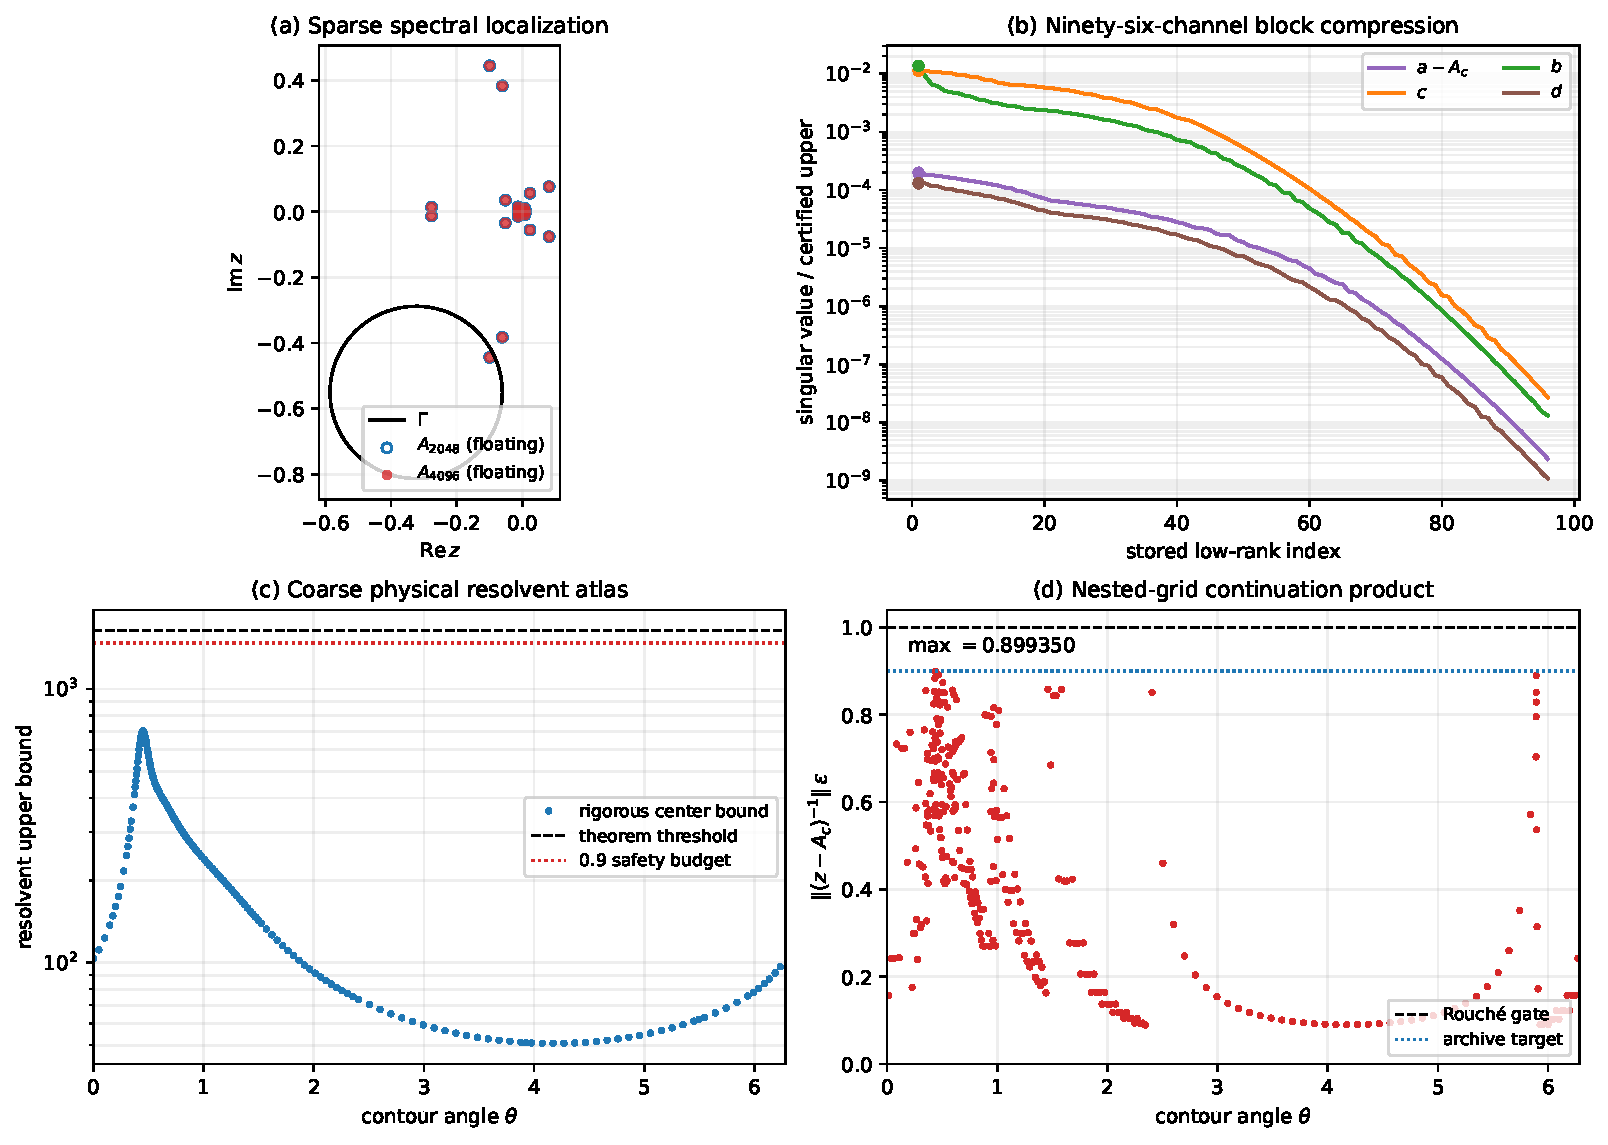
\includegraphics[width=\textwidth]{figures/nested_grid_physical_count.pdf}
 \caption{Nested-grid certificate.  (a) Floating sparse eigenvalues are shown
 only for localization.  (b) The four stored rank-\(96\) block centers have
 rapidly decaying singular values; the first markers show rigorous final norm
 uppers.  (c) Direct physical center-resolvent bounds remain below the theorem
 threshold.  (d) Every rational leaf satisfies the matrix Rouch\'e gate, with
 maximum \(0.899350\).}
 \label{fig:certificate}
\end{figure}

\section{The nested-grid count theorem}
\label{sec:main-theorem}

\begin{theorem}[Certified \(2048\)-to-\(4096\) count continuation]
\label{thm:main}
For the exact stored binary64 matrices \eqref{eq:physical} at
\(\sigma=10^{-2}\), on the contour \eqref{eq:contour-values},
\begin{equation}
 \boxed{N_{\GammaC}(A_{2048})=N_{\GammaC}(A_{4096})=1.}
 \label{eq:main-count}
\end{equation}
Both counts include algebraic multiplicity.
\end{theorem}

\begin{proof}
The coarse count is one by the bitwise replay \eqref{eq:coarse-count}.
By \cref{prop:detail-zero}, the detail resolvent is analytic on and inside
\(\GammaC\), and its interior count is zero.  Hence the fine determinant has
the exact factorization \eqref{eq:schur-det} throughout the counting domain.

For the effective factor, \eqref{eq:effective} gives
\[
 \mathcal F_{\rm f}(z)=(z\Id-\Ac)-\Delta(z).
\]
On every one of the \(314\) rational leaves, the certified atlas and
\eqref{eq:epsilon} give
\begin{equation}
 \norm{(z\Id-\Ac)^{-1}\Delta(z)}_2
 \le0.8993497428917556<1.
 \label{eq:rouche-final}
\end{equation}
The matrix Rouch\'e theorem therefore preserves the determinant winding and
zero count between \(z\Id-\Ac\) and \(\mathcal F_{\rm f}(z)\)
\citep{GohbergSigal1971,Ahlfors1979}.  Thus
\[
 N_{\GammaC}(\mathcal F_{\rm f})=N_{\GammaC}(\Ac)=1.
\]
Adding the zero detail count through \eqref{eq:schur-det} yields
\(N_{\GammaC}(\Af)=1\).
\end{proof}

\begin{remark}[What the theorem does not use]
The proof does not compare two floating eigenvalue lists, invoke a condition
number of an eigenvector matrix, or assume that a rank-\(96\) approximation is
exact.  Floating arithmetic chooses proof centers.  Every final gate is an
outward inequality for the exact stored matrices.
\end{remark}

\section{Floating localization and reproducibility}
\label{sec:numerics}

A \(24\)-mode sparse eigensolve is archived as a diagnostic.  It resolves one
lower-half-plane eigenvalue inside the contour at each dimension:
\begin{align}
 \lambda_{2048}^{\rm fl}
 &=-0.0993604146537118-0.4442017426458030i,\nonumber\\
 \lambda_{4096}^{\rm fl}
 &=-0.0994035212675019-0.4441920040123497i.
 \label{eq:floating-locations}
\end{align}
Their floating displacement is
\[
 |\lambda_{4096}^{\rm fl}-\lambda_{2048}^{\rm fl}|
 =4.41930\times10^{-5}.
\]
The maximum reported eigenpair residual is below \(10^{-15}\).  These values
are consistent with \cref{thm:main}, but they are not validated eigenvalue
disks and do not enter its proof.

The formal archive contains:
\begin{enumerate}[leftmargin=2em]
 \item a \(35\) MiB compressed snapshot of both exact sparse targets and the
       four stored rank-\(96\) proof centers;
 \item componentwise low-rank residual certificates and hashes;
 \item \(170\) center certificates consolidated in a CSV ledger;
 \item an exact \(314\)-leaf rational contour ledger;
 \item the bitwise coarse-count replay and its \(949\)-leaf inherited ledger;
 \item the final theorem JSON, dependency manifest, tests, and figure data.
\end{enumerate}

All center factorizations are replaceable.  Their sparse LU factors are not
trusted or archived as exact objects.  Only the approximate inverse columns,
their exact-target residual hashes, and the resulting outward bounds define
the proof record.

\section{Scope and next gates}
\label{sec:scope}

The theorem establishes one finite-scale stability step:
\[
 2048\longrightarrow4096
 \qquad(\sigma=10^{-2}).
\]
It does not yet establish any of the following.
\begin{enumerate}[leftmargin=2em]
 \item No bound relates either stored matrix to the exact continuum Gaussian
       integral operator.  General Nystr\"om convergence theory does not supply
       the explicit nonnormal contour constants used here automatically
       \citep{Atkinson1997}.
 \item The block bounds are certified only for one adjacent pair.  A uniform
       estimate in \(n\), or an induction over all dyadic refinements, remains
       open.
 \item The noise width is fixed.  Continuation to
       \(\sigma=4\times10^{-3}\) changes both dimension and packet geometry and
       requires a new resolvent atlas.
 \item The unique fine eigenvalue is counted but not enclosed in a validated
       complex disk.
 \item No self-adjoint generator, prime-power trace formula, zeta-zero
       identification, Hilbert--P\'olya construction, or implication for the
       Riemann hypothesis is obtained.
\end{enumerate}

The next direct experiment is the dyadic step \(4096\to8192\) at the same
noise width.  If the coarse/detail norms continue to decrease while the
physical resolvent remains controlled, the method can begin an empirical
uniformity study.  If a gate grows, the failing inequality identifies the
obstruction.  A stronger route would derive analytic quadrature bounds for
the four Haar-coordinate blocks and combine them with a validated continuum
resolvent estimate.

\section{Conclusion}

The finite physical count at dimension \(2048\) is not an isolated numerical
accident under the first dyadic refinement.  Exact coarse/detail coordinates
reduce the \(4096\)-dimensional problem to a detail factor and an analytic
self-energy acting on the coarse space.  Componentwise rank-\(96\) residual
certificates bound the total effective perturbation by
\(6.11954\times10^{-4}\).  A direct physical resolvent atlas then closes the
full-contour Rouch\'e comparison with product \(0.899350\).

The resulting statement is precise and deliberately finite:
\[
 N_{\GammaC}(A_{2048})=N_{\GammaC}(A_{4096})=1
\]
for two exact stored binary64 matrices at \(\sigma=10^{-2}\).  This supplies a
rigorous first bridge from a one-grid physical theorem toward discretization
stability, while leaving continuum and small-noise limits as separate gates.

\appendix

\section{Coordinate formulas used by the certificate}

For a fine vector \(v\in\mathbb C^{2n}\), the implementation evaluates
\[
 (Rv)_j=\tfrac12(v_{2j}+v_{2j+1}),\qquad
 (Sv)_j=\tfrac12(v_{2j}-v_{2j+1}).
\]
The exact block actions are
\begin{align*}
 E_{\rm cc}x&=R\Af Jx-\Ac x,&
 C_{\rm dc}x&=S\Af Jx,\\
 B_{\rm cd}y&=R\Af Ky,&
 D_{\rm dd}y&=S\Af Ky.
\end{align*}
Their Euclidean adjoints are evaluated by reversing the maps and applying the
stored adjoint physical actions.  Unit tests compare all four actions and
adjoints with dense synthetic formulas and independently test the Schur
determinant identity.

\section{Outward arithmetic assumptions}

The componentwise graph assumes IEEE binary64 round-to-nearest arithmetic,
finite intermediate values, no overflow, and no harmful underflow.  Sparse
and dense dot-product errors use conservative operation-count factors in the
standard model of \citet{Higham2002}.  Positive scalar combinations are
rounded one binary64 step outward; circular geometry and final comparisons
use \(256\)-bit Arb.  Exact packet Gram entries are dyadic rationals computed
with integer arithmetic.  These assumptions and the stored object hashes are
recorded in the dependency manifest.

\section{Reproduction commands}

From the paper directory, the fast archive checks are
\begin{verbatim}
PYTHONDONTWRITEBYTECODE=1 python -m pytest -q -p no:cacheprovider
PYTHONDONTWRITEBYTECODE=1 python experiments/build_archive.py
MPLBACKEND=Agg python experiments/make_figures.py
python experiments/verify_archive.py
\end{verbatim}
The \(170\) center certificates are resumable.  A fresh initial batch is
generated by
\begin{verbatim}
OPENBLAS_NUM_THREADS=1 OMP_NUM_THREADS=1 \
python experiments/run_physical_resolvent_batch.py \
  --initial-grid 64 --workers 8 --chunk-size 256
\end{verbatim}
and unresolved midpoint targets are supplied by the atlas JSON until the
exact partition closes.

\bibliographystyle{plainnat}
\bibliography{references}

\end{document}
